%!TEX root = ../main.tex

\section{Maintaining preprocessor-based product lines}
\label{sec:motivating}

\looseness=-1
Inadequate modularity mechanisms are plaguing many languages and cause many implementation problems. Emergent interfaces are applicable to many situations, where explicit interfaces between code fragments are lacking. While we will hint at many other use cases, to illustrate and explore the idea of emergent interfaces, we look at a scenario that is especially challenging to developers involving non-modular code fragments and variability: preprocessor-based product lines.

Variable systems, especially in the form of software product lines, are challenging, because code fragments are configurable and may not be included in all product configurations. That is, developers need to reason about potentially different control and data flows in different configurations. At the same time, when variability is implemented with preprocessor directives, code fragments belonging to a feature are marked (annotated) but not encapsulated behind an interface. Therefore the control and data flow across feature boundaries is implicit (but common, as we found in a previous study~\cite{ribeiro-feature-dependencies-gpce11}).
Industrial product lines can easily have hundreds of features with a large number of possible derivable products. When maintaining a product line, the developer must be sure not to break any of the possible products (as we illustrate next with two scenarios), but due to the sheer number of them, rapid feedback by testing is not possible for all products.

%In this paper, we focus on an Emergent Interfaces integration with preprocessors. In this context, we lack a way to provide better separation of concerns. To follow our idea of evaluating tool-based support to improve modularization, we combine our technique with Virtual Separation of Concerns (VSoC), which allows us to hide feature code not relevant to the current task. This is important to reduce some preprocessor drawbacks and provide better support for feature comprehension. The idea consists of providing developers a way to focus on a feature without the distraction brought by other features~\cite{christian-second-chance-jot09}. However, VSoC is not enough to provide feature modularization, which also aims to achieve changeability~\cite{parnas-criteria-cacm72}. To better illustrate some problems when maintaining two preprocessor-based product lines even with the VSoC support, we present two motivating scenarios.

\subsection{Scenario 1: Implementing a new requirement}
\label{sec:incomplete}

The first scenario comes from the \textit{Best Lap} commercial car racing game\footnote{\url{http://www.meantime.com.br/}} that motivate players to achieve the best circuit lap time and therefore qualify for the pole position. Due to portability constraints, the game is developed as product line and is deployed on 65 different devices~\cite{vander-phd-thesis}. The game is written in Java and uses the Antenna c-style preprocessor.\footnote{\url{http://antenna.sourceforge.net/wtkpreprocess.php}}

To compute the score, developers implemented the method illustrated in Figure~\ref{fig:arena-example}: variable \texttt{totalScore} stores the player's total score. Next to the common code base, the method contains optional code that belongs to feature \emph{ARENA}. This feature publishes high scores on a network server and, due to resource constraints, is not available in all product configurations.

\begin{figure}[h]
    \centering 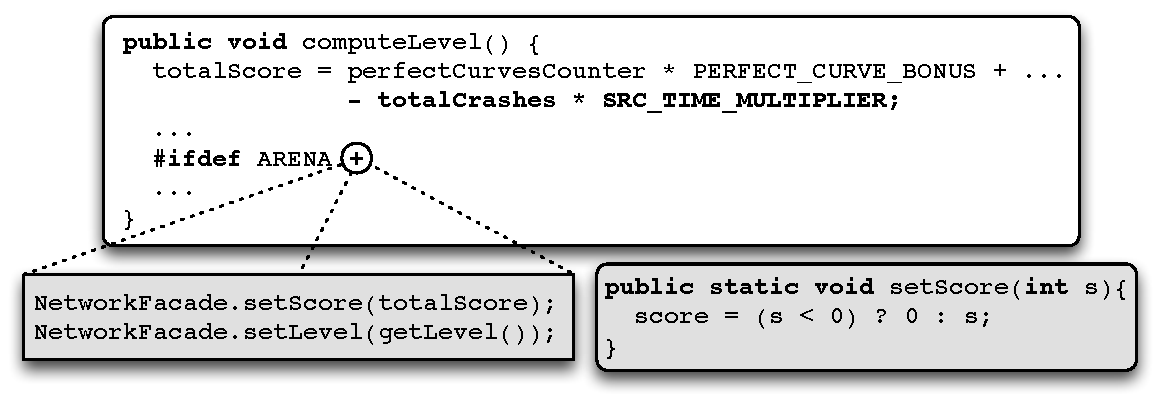
\includegraphics[width=0.5\textwidth]{images/Arena-Example.pdf}
    \caption{Code change only works for some products. \textit{ARENA} feature code in gray.}
    \label{fig:arena-example}
\end{figure}

In this scenario, consider the following planned change.
To add penalties in case the player often crashes the car, let the game score be not only positive, but also negative. To accomplish the task, a developer localizes the \textit{maintenance points}, in this case the \texttt{totalScore} assignment, and changes the computation of scores (see the bold line in Figure~\ref{fig:arena-example}). Products without the \emph{ARENA} feature now enjoy the new functionality, but unfortunately the change is incomplete for products with the \emph{ARENA} feature. In the implementation of feature \emph{ARENA}, method \texttt{setScore} again checks for positive values and unintentionally prevents submitting negative scores to the network server.

The cause of the problem is that the \emph{ARENA} implementation extends the behavior and is therefore affected by the change as well. This was not, however, noticed by the developer, who did not realize that she had to change code associated to other features. In this case, she would have to change part of the \emph{ARENA} code to not check the invariant that all scores are positive. In the actual implementation, feature \emph{ARENA} is partially implemented inside method \texttt{computeLevel} and guarded with \texttt{\#ifdef} directives, so it might not be so difficult to notice the dependency if the method is not so big. 
However, in more complex code or even alternative implementation approaches that separate the feature implementation (see Section~\ref{sec:otherimpl} below) the dependencies across feature boundaries might be harder to track.
%However, we could alternatively implement it in a separate aspect, or keep it hidden through the use of virtual separation. In both cases, for code change tasks that do not obviously relate to feature \emph{ARENA}, the developer could easily miss the dependency.

In this context, searching for cross-feature dependencies might increase developers effort since they have to make sure that the modification does not impact other features. Further, if they miss a dependency, they can easily introduce errors by not properly completing the code change task, for example.

%Building a product with the \textit{ARENA} feature enabled and running it may make the developer incorrectly assume that everything is correct, since the negative total score correctly appears after the race. However, when publishing the score on the network, she notices that the negative score is in fact stored as zero (see the expanded \textit{ARENA} code in gray). Hence, the maintenance was only correctly accomplished for products without \textit{ARENA}.

%The method contains a hidden optional feature, named \textit{ARENA}, responsible for publishing the scores obtained by the player on the network so that players are able to compare their results.

%Also, suppose that the developer is using VSoC, so that there are hidden features throughout the code, including \textit{ARENA}. The developer might well judge that they are not important for this current task. 
%\chk{the following is partially redundant. shorten?}
%So, the developer might be unaware that another feature she is not maintaining uses \texttt{totalScore} and thus also needs to be changed accordingly to correctly accomplish the task. In fact, the impact on other features leads to two kinds of problems. Firstly, due to the incomplete task---the developer should also remove the check from the \texttt{setScore} method---she introduced an \textit{error}. Now, we can only detect this error when we eventually happen to build and execute a product with the problematic feature combination (here, any product with \textit{ARENA}). Secondly, searching for uses of \texttt{totalScore} might increase developers \textit{effort}. Depending on the number of hidden features, the developer needs to consider many locations to make sure the modification did not impact other features. So they might navigate throughout different methods and even different classes, increasing effort.

\subsection{Scenario 2: Fixing an unused variable}
\label{sec:breaks}

Our second scenario is based on a bug report from \textit{glibc}.\footnote{\url{http://www.gnu.org/s/libc/}} This project is structured with several preprocessor macros and conditional-compilation constructs. Developers report that a variable \texttt{status} in the common code base is reported as unused. Investigating the problem, we find that \texttt{status} is declared in all configurations, but only used when features \emph{CHOWN} or \emph{UTIMES} are selected, as shown in Figure~\ref{fig:gfilestatus-example} (left-hand side). When we compile the product line without either feature, the compiler issues an unused-variable warning. 

\begin{figure}[htp]
    \centering 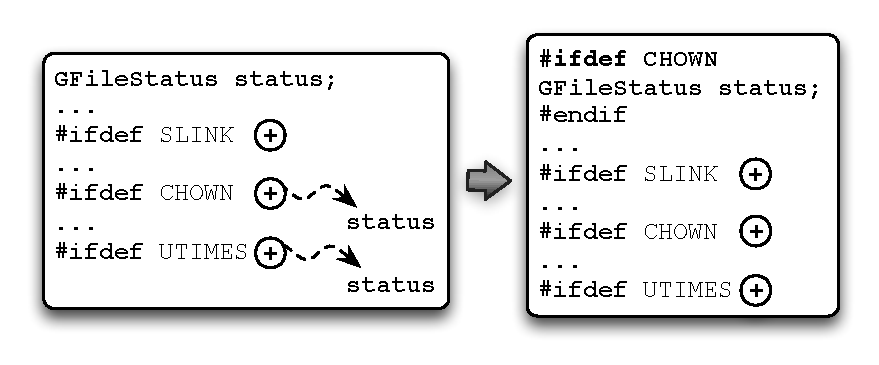
\includegraphics[width=0.4\textwidth]{images/GFileStatus-Example.pdf}
    \caption{Wrong fixing of an unused variable.}
    \label{fig:gfilestatus-example}
\end{figure}

To fix the bug report, a developer would typically look for uses of the variable. If she does not carefully look across feature boundaries, she can easily introduce an error. The problem can even be worse when there are requirements-level dependencies between features, e.g., that \emph{SLINK} cannot be selected without \emph{CHOWN}.

In an unsuccessful attempt to fix the warning, the developer could, for example,  detect only the variable usage in feature \emph{CHOWN}, and then guard the declaration correspondingly as shown in the right-hand side of Figure~\ref{fig:gfilestatus-example}. This would actually lead to a worse problem: an undeclared variable compilation error for configurations with \emph{UTIMES} but without \emph{CHOWN}. The correct fix would require to guard the declaration with \texttt{\#ifdef (CHOWN || UTIMES)}.

%In fact, she solved the unused variable problem but introduced a worse problem: now there is an undeclared variable. Indeed, if we build a product without feature \textit{CHOWN}, we remove the \texttt{status} declaration. Since feature \textit{UTIMES} uses it, the code does not compile for products that contain this feature.

Again, the initial problem and the incorrect fix are caused by the difficulty to follow dependencies across feature boundaries. Again, these are easy to detect in small and simple methods, but might be complicated in larger code bases and other language mechanisms that actually separate the feature code (see Section~\ref{sec:otherimpl} below).

 %This applies not only to preprocessor-based systems and virtual separation environments, but also to systems and product lines structured with other mechanisms. So, in the presence of crosscutting features, identifying feature dependencies may require substantial effort, and missing such dependencies can easily lead to programming errors.

%Because developers can still compile products without the \textit{UTIMES} feature, they did not notice the problem and might generate a release containing it, introducing an \textit{Error} visible only in some out of many configurations, possibly detected only late. Searching for uses of \texttt{status} increases \textit{Effort}.

\subsection{Cross-Feature Dependencies in the Wild}

Initially, the previously shown examples seem pretty specific, requiring preprocessor directives and data-flow dependencies. To quantify their frequency, we have previously conducted a conservative study~\cite{ribeiro-feature-dependencies-gpce11} mechanically mining the code base of $43$ highly configurable software systems with a total of over 30 million lines of code, including \textit{Linux}, \textit{Freebsd}, \textit{postgres}, \textit{sendmail}, \textit{gcc}, and \textit{vim}. All these common open-source systems make heavy use of preprocessor directives for configuration (for features and portability).
Even just looking conservatively at \textit{intraprocedural} data-flow within individual methods, between 1 and 24~percent of all methods in the studied systems contain cross-feature dependencies; however, typically more than half of the methods with \texttt{\#ifdef} directives also contain cross-feature dependencies. These numbers only serve as a lower bound, since \textit{interprocedural} data-flow between methods was not measured but likely causes additional cross-feature dependencies. These results show that the problem, even though quite specific, is so common in practice that building dedicated tool support can be beneficial for a wide range of code change tasks.


%\textbf{TODO: can you add a paragraph or two about the key insights from the GPCE paper?}

\subsection{Beyond preprocessors}
\label{sec:otherimpl}
%Furthermore, code dependencies may cross feature boundaries, so that a variable changed in one feature is read by another feature. A developer must make sure that all of those dependencies are considered as well.

We illustrate the problem for preprocessor-based product lines, but in fact other implementation approaches suffer from limited modularity mechanisms, especially implementation approaches supporting some form of crosscutting. While variability can make cross-feature dependencies harder to detect, it is by no means necessary.

One of the well-known and controversially discussed examples is \emph{aspect-oriented programming} in the style of AspectJ. With AspectJ, code of features (or more generally concerns) is separated into a distinct code unit, the aspect, and reintroduced in a weaving step. The control-flow or data-flow between aspects and base code is not protected by explicit interfaces---a fact for which AspectJ was repeatedly criticized~\cite{storzer-fragile-pointcut-04, S:OOPSLA06}, but which was also discussed as strength enabling flexibility~\cite{filman:oopsla-aop00}.%
\footnote{Several extensions to aspect-oriented languages have been discussed that require declaring explicit interfaces between concerns~\cite{SPAK:TOSEM10,join-point-interfaces-erics-esec-fse11,aldrich-open-modules-ecoop05,GSSSTCR:IEEESoftware06,rajan-ptolemy-ecoop08}; here we take an alternative tool-based approach.} The first example works just as well with an aspect injecting the \emph{ARENA} code instead of an in-place \texttt{\#ifdef} block.

Other structure-driven composition mechanisms, such as \emph{feature-oriented programming}~\cite{batory-refinement-tse04}, \emph{delta-oriented programming}~\cite{delta-ina-splc10}, or even just inheritance with \emph{subclassing}~\cite{fragile-base-class-ecoop98} exhibit similar potential problems.

Finally, also in the context of preprocessor-based implementations, recent advances support some separation of feature code.
To deal with the scattering of feature code in preprocessor-based implementations, researchers have investigated \emph{virtual} forms of separating concerns by helping developers to focus on relevant features~\cite{christian-cide-icse08,ABGM:TSE02,erwig-harmful,HKW:ICSE08}. For example, in CIDE~\cite{christian-cide-icse08}, developers can create \emph{views} on a specific feature selection, hiding irrelevant files and irrelevant code fragments inside files, with standard code-folding techniques at the IDE level. Code fragments are hidden if they do not belong to the selected feature set the developer has selected as relevant for a task. In our examples, we have already shown the collapsed versions of \texttt{\#ifdef} statements with a $\oplus$ marker indicating additional code. Virtual separation in this form has been shown to allow significant understandability and productivity gains~\cite{ABGM:TSE02,erwig-harmful}. However, hiding also has a similar effect as moving code into an aspect: it is no longer visible locally (except for a marker indicating hidden code) and there is no interface describing the hidden code. This way, virtual separation makes the problem of cross-feature dependencies even worse.




%The problem we outline is shared by many implementation approaches for product lines that support some form of crosscutting. For example, if we use aspects (or similar techniques) to implement crosscutting features~\cite{eduardo-empirical-study-icse08}, and configure the product line by selecting which aspects to weave, we need to consider potential dependencies between (optional) aspects and classes. In practice, a more common scenario, and the one we focus here, is to use conditional-compilation (\texttt{\#ifdef} constructs) with a preprocessor, where optional code fragments are merely annotated in a common code base~\cite{liebig-40spls-icse10}. Also in this context, dependencies cross method and feature boundaries and may only occur in specific configurations and are not explicit in interfaces.

%To deal with the scattering of feature code in preprocessor-based implementations, researchers have investigated virtual forms of separating concerns by helping developers to focus on relevant features. For example, in CIDE~\cite{christian-cide-icse08}, developers can create views on a specific feature selection, hiding irrelevant files and irrelevant code fragments inside files, with standard code-folding techniques at the IDE level. Code fragments are hidden if they do not belong to the selected feature set the developer has selected as relevant for a task. While virtual separation with hiding can emulate some form of modularity, it also potentially hides code fragments that might be relevant for code change tasks. Similar to separating features with aspects, a view shows only the code of one feature (or a set of features) while dependencies may point to code in other aspects or hidden code fragments (visible only in other views). Developers are then prone to make errors and need to invest effort to trace dependencies, as we illustrate next with two scenarios.